\chapter{Applications robotiques complexes}
\label{chap:integration}

\epigraph{Text text text text text text text text text text text text
  text text text text text text text text text text text text text
  text text text text text text text text text text text text text
  text text text text text text text text text text text text text
  text text text text}{Some Author}
\clearpage

\lettrine[lines=2, lraise=0.1, nindent=0em, slope=-.5em]%
{C}{e} chapitre est dédié à la conception d'architectures robotiques
complexes permettant la validation de nouveaux algorithmes robotiques.
Les précédents chapitres ont montré une progression d'une approche
qui est dédiée purement à la génération de trajectoires via
l'utilisation d'outils d'optimisation numérique vers un l'exécution de
scénarios dont la complexité a augmenté incrémentalement. Ce passage
de la génération de trajectoire sans ``conscience'' de ce qu'est un
système évoluant dans le monde réel vers une application robotique
réelle ne va pas sans la nécessité d'intégrer et de maîtriser une
grande variété d'algorithmes et de technologies tout en les utilisant
conjointement afin de finalement, atteindre un objectif de haut
niveau. Ce chapitre va donc décrire l'architecture qui a été mise en
place sur le robot humanoïde HRP-2 afin de réaliser un ensemble de
scénario expérimentaux, certains faisant partie intégrante des
chapitres précédents et d'autres étant le résultat de travaux de
recherche disjoints mais prenant appui sur l'architecture développée
ici. Ce chapitre tente également de fournir des conseils et une
méthodologie pour la conception d'applications robotiques. Une partie
de la méthodologie décrite dans ce chapitre est issue des
recommandations classsiques de l'ingénierie logicielle mais il est
également nécessaire de prendre en considération les particularités de
la robotique.

\section{Architecture}


Les systèmes robotiques complexes peuvent être décomposé en trois
grandes parties:

\begin{enumerate}
\item La couche de perception\index{perception} qui analyse
  l'environnement autour du robot et construit un modèle du monde,
\item La couche de décision\index{décision} qui va tenter de résoudre
  la tâche donnée au système tout en prenant en compte l'état actuel
  du monde,
\item La couche action\index{action} qui va utiliser les capacités du robot pour
  réaliser la tâche proprement dite. En particulier, les capacités
  d'actionnement du robot sont ici utilisées pour impacter le monde
  environnant.
\end{enumerate}


Cette architecture largement décrite par la littérature est encore
d'actualité pour les robots humanoïdes. En effet, cette catégorisation
est issue de la présence dans un système robotique de boucles lentes
et de boucles rapides. Typiquement, la prise de décision est un
processus lent -- qui peut prendre plusieurs secondes --, la
planification de mouvements est un exemple de ce type de processus. Au
contraire, la couche action contrôlant les actionneurs nécessite le
plus souvent d'être extrêmement réactive et impose des contraintes
importantes en terme de temps réel. Il faut pouvoir garantir que la
boucle de contrôle peut être évaluée à une fréquence donnée ce qui
contraint à la fois le type d'algorithmes pouvant être exécuté dans
cette boucle ainsi que le volume de donnée pouvant être traité. Enfin,
la couche de perception est elle, en général plus lente que le
contrôle et dépendante de la vitesse à laquelle les capteurs du robot
peuvent fonctionner. Qui plus est, il arrive parfois que les capteurs
acquièrent des données plus vite qu'elles sont traitées et certains
données sont alors ignorées silencieusement. On a donc ici trois types
de comportements extrêmement différents.


Les couches perception et décision nécessitent une grande puissance de
calcul pour pouvoir assurer une réactivité suffisante. Cette puissance
de calcul est parfois déportée sur un ordinateur spécifique. Par
exemple dans le cadre du robot HRP-2, deux ordinateurs sont
embarqués. Le premier est dédié à la boucle de contrôle temps réel et
est relié aux actionneurs tandis que le second est relié aux capteurs
-- ici les caméras embarquées -- et support les algorithmes de
décision et de perception.


Afin de découpler les algorithmes robotiques, chaque algorithme est
implémenté au sein d'un composant robotique\index{composant
  robotique}. En pratique, un composant robotique est un processus --
c'est à dire un programme indépendant -- pouvant communiquer avec un
ou plusieurs autres composants. La distribution des calculs sur
plusieurs ordinateurs rend nécessaire la définition d'un protocole de
transmission des données afin de pouvoir assurer une bonne
interprétation de ces dernières au sein d'un environnement
informatique hétérogène. Un exemple est la représentation des nombres
au sein des architectures informatique: une architecture peut être
dîte ``big endian''\index{big endian (architecture)} ou ``little
indian''\index{little endian (architecture)} selon l'ordre dans lequel
les bits représentants le nombre sont enregistrés. Dans une
architecture ``big endian'' les nombres aillant les poids les plus
forts sont contenus en mémoire en premier tandis que les architectures
``little endian'' adoptent un ordre inverse. Ce type de problème rend
nécessaire la définition d'un modèle de communication entre
composants.


Les architectures robotiques autorisent généralement la communication
entre deux composants, ou n\oe uds, soit sous une forme discrète, soit
sous une forme continue. La forme discrète est appelée
``service''\index{service} et se modélise sous la forme d'un appel de
fonction distant. Un algorithme est généralement divisé en fonctions,
ces dernières formant des blocs logiques pouvant être combinés entre
eux pour réaliser des comportements de plus haut niveau. Les services
fournissent un moyen d'appeler une fonction qui ne sera non pas
exécutée au sein du processus courant mais dans un autre processus,
voire sur un autre ordinateur de manière transparente. La difficulté
résidant dans le passage des arguments et la transmission du
résultat. Il est nécessaire que cette fonction soit défini selon des
règles particulières afin de s'asssurer que les données peuvent être
correctement transmises via la réseau sans compromettre leur
intégrité. Cette phase dîte de ``sérialisation''\index{sérialisation}
assurer le fonctionnement de ces méchanismes dans des environnements
informatiques hétérogènes. La seconde forme de communication sert à
modéliser des flux de donnée continus et est appelé
``topic''\index{topic}. Dans ce cas, le premier composant communique a
un ou plusieurs autres des données mises à jour régulièrement. De la
même façon, un processus de sérialisation est nécessaire pour assurer
que les données peuvent être transmises même si un ou plusieurs autres
composants ne font pas parti du même processus ou ne sont pas exécutés
sur le même ordinateur.


De nombreux outils logiciels implémentent ces méchanismes sous
différentes formes. Le choix réalisé sur le robot humanoïde HRP-2 a
été d'utiliser ROS -- Robotics Operating System --\index{ROS}, un
projet communautaire initié par la société californienne Willow
Garage\index{Willow Garage}. Le méchanisme de communication ainsi
qu'une grande partie de la modélisation du processus de perception se
fonde sur les outils développés dans le cadre de ce projet. Les
sections suivantes vont détailler les différents composants
fonctionnant sur le robot humanoïde HRP-2.



\subsection{Contrôle}

Sous le terme de ``contrôle'' est désigné le composant robotique
chargé de calculer la commande qui sera envoyée aux actionneurs. Il
est impératif que cette ordre déterminant le prochain état que les
servo-moteurs du systèmes vont s'efforcer d'atteindre, soit envoyé à
une fréquence fixe. Sur le robot humanoïde HRP-2, la fréquence de la
boucle de contrôle est de 200 Hz, il faut donc que la boucle de
contrôle ne mette pas plus de 5ms pour être évaluée. Les noyaux des
systèmes d'exploitation multi-tâches ne fournissent pas de garantie
forte sur la réactivité des logiciels exécutés. Il est donc nécessaire
d'utiliser des noyaux dédiés afin d'assurer que la boucle de contrôle
soit exécutée en permanence à la fréquence voulue. Ces contraintes
impliquent que les composants de contrôle se doivent d'être aussi
minimaux que possible et sont souvant monolitiques. À ce sujet, les
contrôleurs robotiques partagent une grande ressemblance avec les
noyaux des systèmes d'exploitation. Ils assurent également la sûreté
du système: une mauvaise commande envoyée aux moteurs peut, très
souvent, entraîner la destruction des actionneurs.

Dans le cas de systèmes robotiques complexes, il est courant d'avoir
plusieurs contrôleurs exécutés successivement au sein de la boucle de
contrôle. Ainsi l'architecture d'HRP-2 se fonde sur un système de
plug-in permettant de charger des contrôleurs ``à chaud''. Chaque
contrôleur est alors modélisé par une machine à état très simple FIXME
FIG. Le contrôleur passe alors dans les états suivants:

\begin{itemize}
\item Initialisation sans contrainte de temps réel
\item Initialisation avec contrainte de temps réel
\item Exécution
\item Destruction avec contrainte de temps réel
\item Destruction sans contrainte de temps réel
\end{itemize}

Le passage d'un état à l'autre se réalisant dans l'ordre, avec un
bouclage sur la phase d'exécution autant qu'il est nécessaire.


L'architecture de contrôle est divisée en trois contrôleurs:
\begin{description}
\item[Pile de tâches\index{piole de tâches}] À partir d'un ensemble de
  tâche, la résolution de la pile de tâche est calculée dans la boucle
  de contrôle afin de calculer la commande à envoyer aux
  moteurs. HRP-2 étant commandé en position, la commande envoyée
  correspond à la position articulaire des différents joints du
  système.
\item[Stabilisateur\index{stabilisateur}] HRP-2 intègre un méchanisme
  d'absorption passif des chocs appelé ``silent blocks''\index{silent
    block}. Ce système passif intègre au niveau des chevilles une
  compliance difficile à modélisée et à prendre en compte dans le
  calcul de la commande. La centrale inertielle du robot permettant
  d'estimant l'attitude du bassin, le stabilisateur peut déduire
  l'état des flexbilités des chevilles et, à l'aide des capteurs de
  force placés dans les cheville, réaliser un asservissement
  bas-niveau sur la trajectoire du ZMP désiré. Ce méchanisme permet de
  compenser la modélisation sommaire de la dynamique réalisée, par
  exemple, par l'utilisation du modèle simplifié du ZMP ainsi que des
  éventuelles erreur de modélisation de la structure du robot. Ce
  système compense les erreurs de suivi du ZMP en modifiant les
  valeurs des articulations des jambes du robot.
\item[Communication] Le dernier élément communique vers l'extérieur
  les informations lié au contrôle du robot tel que les commandes
  envoyées, réellements exécutées -- c'est à dire après stabilisation
  --, ainsi que les sorties des capteurs tels que la centrale
  inertielle et les capteurs de forces placés aux chevilles et
  poignets du robot.
\end{description}


On notera que pour le dernier contrôleur, la communication réseau
étant implémentée en TCP/IP\index{TCP/IP}, il n'est pas possible de
garantir le temps pris par l'envoi des données et il est donc
impossible d'envoyer des données en TCP/IP\index{TCP/IP} sans
compromettre la boucle temps réel. Cette partie est donc divisée en
plusieurs fils d'exécution non-bloquants afin de garantir la sûreté du
système. En pratique, chaque ``topic'' permettant la communication de
données vers l'extérieur publie les données dans un fil d'exécution
séparé et non temps-réel. Le fil d'exécution\index{fil d'exécution}
temps réel lui tente de copier la donnée vers une variable lue par ce
fil d'exécution. Si ce dernier est en train d'y accéder et qu'elle
n'est pas accessible, un verrou protège l'accès à la ressource et la
publication de la donnée pour ce tour de boucle est ignorée. En
pratique, la communication vers l'extérieur est réalisée à 20Hz. En
moyenne, une donnée sur dix est donc envoyée afin d'éviter d'engorger
le système.


En terme de conception, les composants nécessitant un rafraichissement
à une vitesse supérieure doivent être intégré à la boucle de
contrôle. Pour les autres données, il faut pouvoir, via le schéma de
calcul, pouvoir utiliser les informations temporelles attachées aux
données capteur envoyées pour gérer de manière consistante le retard
inhérent à toute donnée provenant d'une architecture distribuée.


\subsection{Vision}


La vision est l'élément central de la perception sur un robot
humanoïde. Elle est caractérisée par une particularité qui détermine
tous les traitements qui lui sont affectés: les caméras produisent des
quantités de données extrêmement importantes. De ce fait, il est
important d'éviter de réaliser des traitements inutiles et il faut
également éviter au maximum les copies. Le traitement des images est
souvent réalisé en série: on acquiert une image, on la convertit, on
la rectifie et puis on chercher à en tirer des informations de plus
haut niveau. Ces traitements en série se modélisent particulièrement
bien sous la forme d'un tuyau dans lequel les images passent les unes
après les autres. La stratégie classique de la robotique tend alors à
dédier un composant par traitement afin de garder un système
modulaire, mais la taille des données rend cela difficile. En effet,
si chaque composant vit dans un processus différent, il est nécessaire
de passer par des méchanismes de mémoire partagée afin d'éviter les
copies en mémoire. ROS a choisit une seconde stratégie en offrant la
possibilité d'agglomérer plusieurs composants dans un seul
processus. La sérialisation devient donc totalement inutile au prix
d'une plus grande complexité dans l'écriture des n\oe uds et d'une
forme d'insécurité: si un problème advient dans n'importe lequel de
ces composants, il provoquera l'arrêt de la totalité du
système. Cependant, les traitements étant effectués en série, devoir
relancer tous les traitements en cas de panne n'amène pas de perte
significante de qualité de service.


Nous allons donc désormais nous attacher à développer les différents
composants de vision qui ont été utilisé sur le robot HRP-2 et
aggloméré dans la chaîne de traitement des images du robot.


\paragraph{Acquisition des images}

L'acquisition des images est réalisée par un composant communiquant
avec le pilote FireWire. Les quatre caméras du robot sont des Flea2 du
fabriquant PointGrey. Ces caméras sont reliées à un FireWire IEEE
1394b\index{FireWire IEEE 1394b}. Les limitations du bus ne permettent
pas l'acquisition des données sur les quatre caméras simultanément, on
peut donc passer de la paire de caméras grand angle à la seconde paire
de caméras. La première paire est dédiée à la perception de
l'environnement au détriment de la précision tandis que la seconde
dispose d'un champ plus resserré, adapté à la manipulation fine
d'objets notamment.

Les images acquises utilisent un encodage de Bayer\index{Bayer
  (encodage de)}. Cet encodage, nommé du nom de son inventeur, Bryce
E. Bayer chercheur au sein de la société Kodak, réalise l'encodage
d'images couleurs sur 8 bits au lieu des 24 bits habituellement
nécessaires pour représenter les trois canaux utilisés pour encoder
les trois couleurs primaires: rouge, vert et bleu. Cet encodage encode
la couleur verte sur 50\% du volume de donnée totale tandis que bleu
et rouge représentent 25\% chacun. Cette prépondérence du vert est
fondé sur la plus grande sensibilité au vert des cônes, les
photorécepteurs présents au fond de l'\oe il.


\paragraph{Traitements des images}

Une fois les images acquises, il est important de les convertir dans
un espace colorimétrique\index{espace colorimétrique} adapté à leur
traitement. La première étape est donc de dématricer les images
encodées en Bayer vers des images monochromatiques ou couleurs 24 bits
dans l'espace RGB habituel. Dès maintenant, un branchement s'effectue
entre les traitements utilisant les images couleurs et les traitements
utilisant les informations de luminance uniquement. Afin de fournir
une expérience unifiée, les deux ``topics'' sont créés, mais les
traitement ne sont effectués qu'à partir du moment où au moins un
client se connecte à ce dernier. On peut donc offrir une large palette
de possibilités sans mettre à mal les performances du système. Le
dématriçage\index{dématriçage} des images encodées en Bayer
reconstruit les couleurs manquantes en interpolant grace à la couleur
des pixels adjacents. Plusieurs techniques aillant des coûts de calcul
différents existent selon les cas: interpolation bilinéaire,
interpolation bicubique ou bien encore rééchantillonage de
Lanczos\index{Lanczos (rééchantillonage de)}.


La seconde étape consiste à rectifier les images. Nous nous
intéresserons d'abord au cas de la rectification\index{rectification}
monoculaire. Dans ce cas, l'objectif de ce procédé est de se ramener
au cas de la caméra parfaite dîte
``pinhole''\index{sténopé}\index{modèle de caméra
  pinhole|see{sténopé}} -- ou sténopé en français -- où la projection
du point 3d $P$ sur le plan image donne un point 2d $p$ qui correspond
parfaitement à la projection de ce dernier en passant par le point
focal de la caméra $C$: $p_x = P_x / P_z$ et $p_y = P_y / P_z$ où
$P_x, P_y, P_z$ sont les coordonnées du point dans l'espace 3d et
$p_x, p_y$ les coordonées 2d du point $p$ dans le plan image. Ce n'est
pas jamais totalement le cas en réalité: le plan image n'est pas un
plan parfait, l'axe optique n'est jamais exactement au centre de la
caméra et les objectifs réalisent une distorsion\index{distorsion} des
rayons lumineux captés. Pour pouvoir raisonner sur ce modèle idéal, on
va donc traiter l'image afin qu'elle puisse être considérée comme
provenant d'un capteur idéal aillant le comportement d'un sténopé, à
la différence de la caméra réelle. Il faut pour cela calibrer la
caméra et identifier ses paramètres intrinsèques\index{paramètres
  intrinsèques (de caméra)}: $(u_0, v_0)$ la position de l'axe optique
dans l'image, $(p_x, p_y)$ la taille des pixels permettant de réaliser
la conversion des pixels vers les mètres et un ensemble de paramètres
permettent d'identifier la distorsion de l'image originale. Plusieurs
modèles sont décrits par la littérature, mais dans notre cas une
estimation de la distorsion radiale\index{distorsion radiale} est
suffisante pour compenser l'utilisation d'un objectif grand angle.


Le processus de calibration est réalisé en utilisant une mire que l'on
place à différents endroits relativement à la caméra. Connaissant la
taille des points et leur écartement, on peut alors, via la résolution
d'un problème type moindre carrés linéaires, réaliser une estimation
des paramètres intrinsèque des caméras du système.

Une fois de plus, ce traitement est disponible dans deux variantes
différentes: monochromatique et couleur.

\begin{figure}
  \begin{center}
    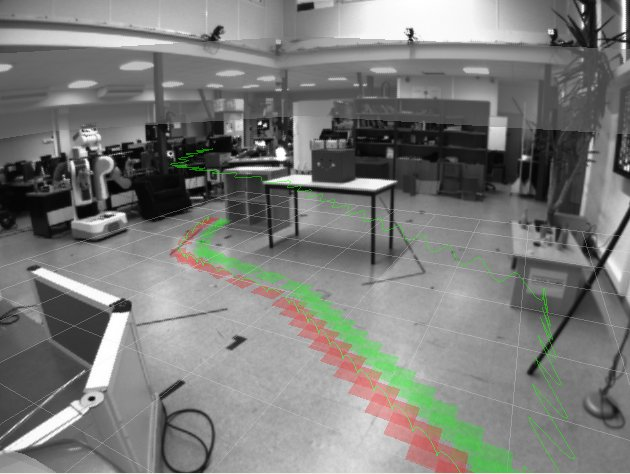
\includegraphics[width=.95\linewidth]{src/chap4-integration/footsteps2.jpg}
  \end{center}
  \caption{Affichage de la pile de pas que le robot va réaliser en
    réalité augmentée.}
\end{figure}



\paragraph{Vision stéréoscopique}\index{vision stéréoscopique}


Le dernier traitement concernait la vision monoculaire. Il est
courant, en robotique, d'avoir recours à la vision stéréoscopique afin
de pouvoir reconstruire la profondeur d'un objet visible dans les deux
caméras. Il est alors nécessaire d'estimer la transformation relative
entre les deux caméras afin de pouvoir rectifier l'image de la seconde
image de la paire de caméras stéréo. Via ce processus, les images de
deux caméras sont prises par des capteurs virtuels dans les plans
images sont coplanaires. On peut alors faire en sorte que la
projection d'un point 3d se fasse sur la même ligne tant sur la caméra
de gauche que sur la caméra de droite. Le problème de l'appariement
des points se ramène alors à une problème unidimensionnel de
complexité moindre permettant la construction d'une carte de
profondeur. Cette carte est disponible sous la forme d'un topic, mais
les données de profondeur sont également disponibles sous la forme
d'un nuage de points. Dans ce dernier, on associe à chaque point la
couleur du pixel correspondant dans l'image. Ce topic est
particulièrement utile lorsque l'on souhaite utiliser des algorihtmes
de traitements de nuages de points 3d tel que PCL -- la Point Cloud
Library --\index{PCL (Point Cloud Library)}.


Une fois de plus, la totalité du processus de vision peut fonctionner
dans un processus unique afin d'éviter les copies. Cette architecture,
également adoptée sur le robot PR2\index{PR2 (robot)} de Willow
Garage, fournit donc un compromis intéressant entre rapidité,
souplesse d'utilisation et modularité.

\begin{figure}
  \begin{center}
    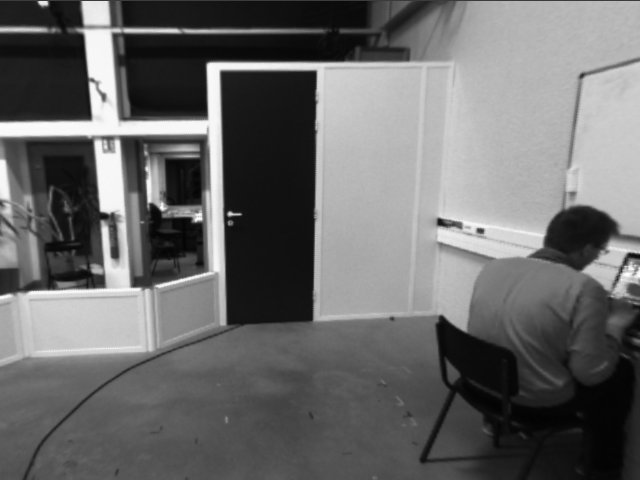
\includegraphics[width=.95\linewidth]{src/chap4-integration/disparity-1.jpg}
    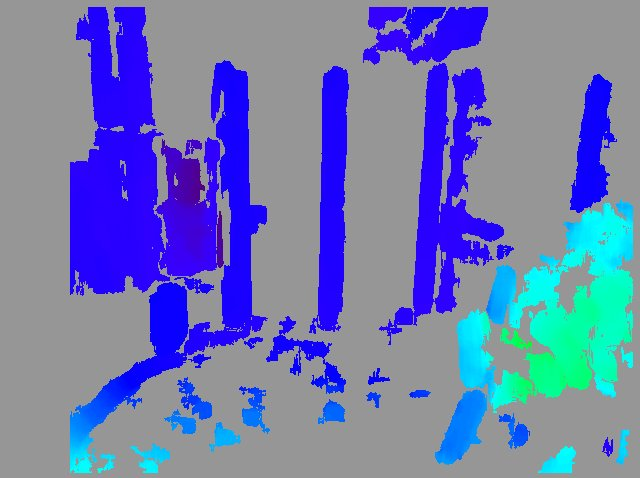
\includegraphics[width=.95\linewidth]{src/chap4-integration/disparity-2.jpg}
  \end{center}
  \caption{Carte de profondeur calculée en temps réel. Une couleur
    claire correspond à une faible profondeur, une couleur foncée à
    une profondeur importante. Les zones grises indiquent les endroits
    où aucune correspondance n'a pu être établie entre les images de
    deux caméras. Elles correspondent typiquement à une zone peu
    texturée comme un mur.}
\end{figure}


\begin{figure}
  \begin{center}
    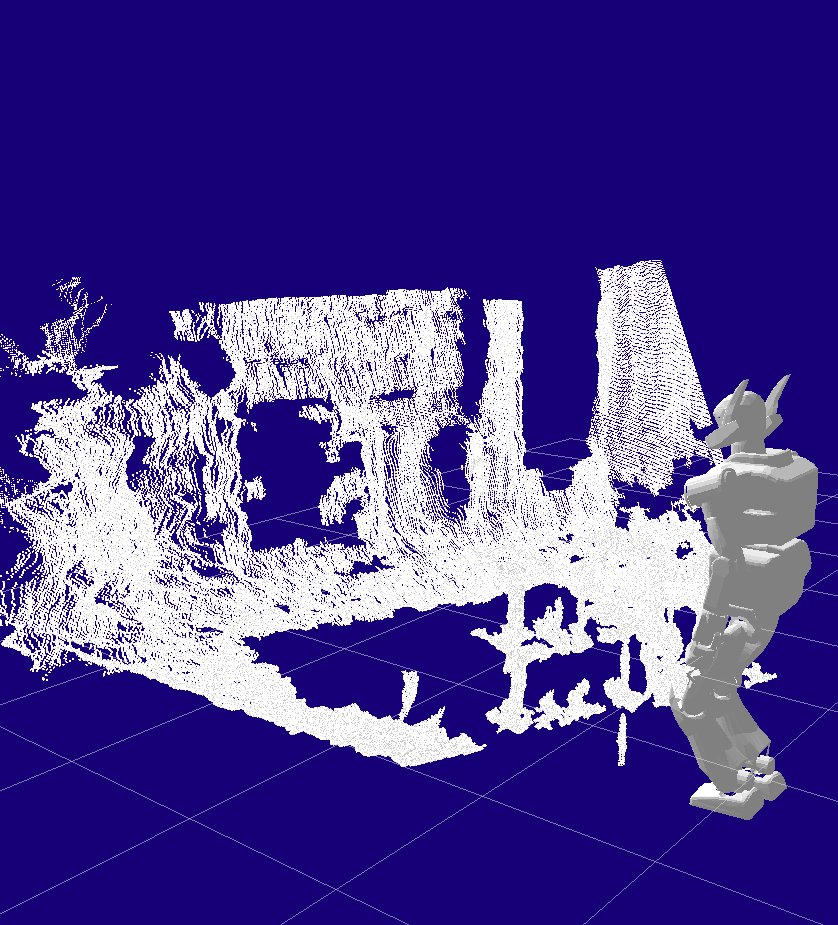
\includegraphics[width=.95\linewidth]{src/chap4-integration/stereo1.jpg}
  \end{center}
  \caption{Reconstruction 3d de l'environnement autour du robot HRP-2
    à partir des données de la paire de caméra stéréo.}
\end{figure}


\subsection{Capture de mouvement}

Une alternative à la vision embarquée est l'utilisation des systèmes
de capture de mouvement. Ces derniers, à l'origine destiné à étudier
les mouvements humains, ont été largement détournés afin de pouvoir
suivre les mouvements d'objets autour du robot et s'abstraire des
difficultés propres à la perception en robotique.


Un composant réalisant l'interface entre d'une part, le système de
capture de mouvement, et l'architecture robotique a été écrit. Ce
dernier permet de suivre les mouvements de plusieurs objets
simultanéments et publie une estimation de leur pose via le système de
``topics'' précédemment décrit.


\subsection{Diagnostics et sûreté}

L'utlisation d'un robot humanoïde de grande taille présente toujours
un risque, et ce dernier tend à croître quand l'architecture devient
plus complexe et intègre des composants moins fiable. Pour se faire,
il est donc nécessaire d'avoir un moyen de pouvoir obtenir un état
complet du système de manière unifiée. Ce dernier est disponible sur
le robot et est illustré par la figure FIXME. De plus, il est
nécessaire à tout moment de pouvoir avoir un retour si le mouvement
exécuté présente le risque d'endommager le robot. Ces risques se
divisent en différentes catégories:
\begin{description}
\item[Endommagement des capteurs] Les capteurs de forces sont conçus
  pour résister à un impact de 1000N au plus. Il est recommandé de ne
  pas aller au-delà de 800N par mesure de sécurité. Les autres
  capteurs ne présentent pas de risque particulier.
\item[Endommagement des actionneurs] Les actionneurs peuvent fournir
  un couple maximal. Au delà de ce dernier, il risque de chauffer de
  manière trop importante et d'être rendu inopérant. On peut donc
  fixer une borne ``raisonnable'' qui ne devrait jamais être
  dépassé. Évidemment, ceci ne représente qu'une approximation très
  simple des capacités maximum des actionneurs. En particulier, un
  retour sur la température des actionneurs se révélerait être un
  indicateur intéressant mais n'est malheureusement pas disponible en
  l'état actuel des capacités du robot.
\item[Instabilité lors de la locomotion] Il est possible d'estimer la
  position du ZMP à partir des forces mesurées par les capteurs de
  force. Cette estimation permet d'avertir l'utilisateur quand le ZMP
  se rapproche dangereusement de la limite du polygone de
  sustentation.
\item[Déviation des horloges des ordinateurs embarqués] Les
  ordinateurs embarqués synchronisent leurs horloges en utilisant le
  protocole NTP -- Network Time Protocol --. L'ordinateur dédié à la
  décision et la perception se synchronize sur un serveur de temps
  distant. L'utilisation d'un lien wifi et la présence de routeurs
  intermédiaires rend la synchronisation relativement peu
  précise. Cependant, le problème n'est pas très grave car le
  véritable enjeu reste de faire en sorte que les deux PCs embarqués
  gardent leurs deux horloges synchronisées. Le lien réseau étant
  direct, la synchronisation relative de ces deux ordinateurs est, au
  contraire, de très bonne qualité et permet d'assurer la cohérence
  des données temporelles entre, d'une part, le contrôleur commandant
  les actionneurs, et d'autre part les composants de décision et de
  perception.
\item[Difficultés informatiques d'ordre général] Au delà des problèmes
  décrits précédemment et qui affectent plus particulièrement les
  systèmes robotiques, les robots sont également affectés par
  l'ensemble des problèmes qui peuvent toucher un ordinateur:
  température excessive du processeur, manque d'espace de stoquage,
  etc.
\end{description}

Une des difficultés de la mise en \oe uvre d'un système robotique est
la nécessité de faire fonctionner un ensemble de technologies
complexes sachant que le mauvais fonctionnement de n'importe quel
morceau de l'architecture peut mettre en péril la tâche tout
entière. Qui plus est, certaines limitations du matériel tel que le
couple maximum des actionneurs est parfois vérifié, a posteriori. Des
systèmes de surveillance des valeurs critiques sur les couples, les
impacts sur les capteurs de force ont donc été mis en place afin
d'éviter d'endommager le matériel.


\section{Simulation transparente}


Une difficulté récurrente en robotique est la lenteur de la
réalisation des expérimentations: calibrer un robot et réaliser une
expérience demande beaucoup de temps. Afin d'accélérer au maximum le
développement et d'assurer la sécurité des expérimentateurs et du
matériel, une phase de simulation des expérimentations reste cruciale.


L'utilisation d'une architecture robotique fondée sur un modèle de
communication donne ici tout son intérêt: la totalité des capacités du
matériel, tant au niveau de l'actionnement que des capteurs est
représenté informatiquement par un ensemble composé de services et de
``topics''. Tant que le simulateur choisit fournit ce même ensemble de
canaux de communication, les algorithmes pourront fonctionner
indiféremment en simulation ou sur le véritable système. Il reste
alors le plus important: assurer la cohérence entre les capteurs
simulés en fonction des commandes envoyées aux actionneurs. Pour se
faire, il est important de disposer d'un moteur physique
réaliste. Dans le cadre de cette thèse, le simulateur OpenHRP a été
choisi. En effet, la plupart des simulateurs robotiques -- Gazebo,
Webots --, utilisent des moteurs physiques primitifs adaptés aux
robots mobiles ne réalisant pas de mouvements ``dynamiques''. Afin de
modéliser précisément les interactions entre le pied et le sol, un
moteur physique disposant d'un modèle de contact convaincant et précis
est indispensable à la simulation d'un mouvement réalisé par un robot
humanoïde.


Les limitations de la plate-forme sont généralement lié à la
simulation des caméras, ne pouvant jamais reproduire les difficultés
inhérentes à la vision par ordinateur: changements d'illumination,
délai induit par l'acquisition et le transfert des données, erreur de
calibration de la caméra, etc. La simulation est donc davantage un
moyen de tester la correction du raisonnement et pas tant un outil
fiable pour démontrer sa robustesse à la réalité qui diverge toujours
du modèle calculé.


\section{Modélisation unifiée d'un système robotique}


La génération de mouvement se fonde sur une connaissance précise des
capacités physiques des robots. Cette description est généralement
encodée à l'aide d'un format de fichier permettant de représenter les
différentes informations caractérisant le système. Une définition
mathématique du système a été donnée dans le chapitre 2 FIXME. Du
point de vue informatique, le format de fichier URDF -- Unified Robot
Description Format --, SRDF -- Semantic Robot Description Format -- et
RCPDF -- Robot Contact Point Definition Format -- est utilisé pour
représenter les informations nécessaires à la génération de mouvements
sur un robot humanoïde. Les deux premiers formats sont le fruit du
travail de la communauté ROS tandis que le dernier a été développé
dans le cadre de cette thèse.

\begin{figure}
  \begin{center}
    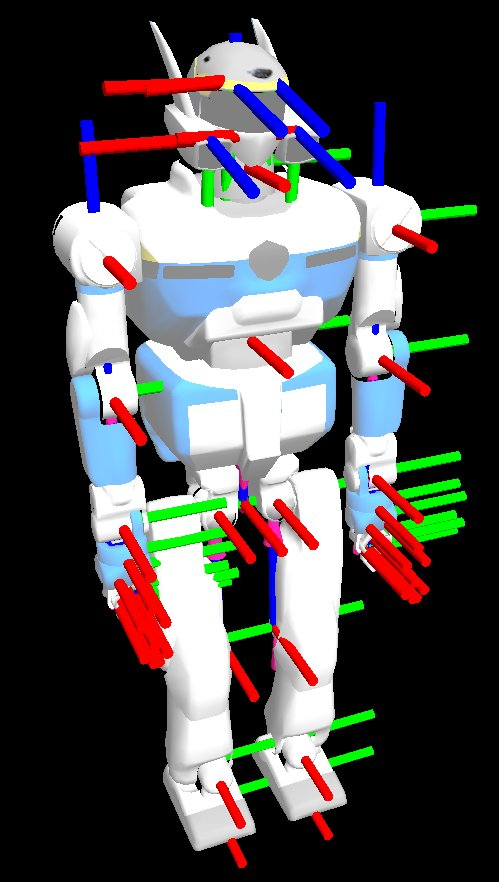
\includegraphics[width=.45\linewidth]{src/chap4-integration/hrp2_urdf.jpg}
  \end{center}
  \caption{Modèle de robot HRP-2 décrit via le format URDF.}
\end{figure}



\subsection{Description d'un robot}


Un robot est un ensemble de corps dont les mouvements relatifs sont
contraints. La modélisation des contraintes passe par la modélisation
des articulations reliant deux corps entre eux. Le format URDF définit
donc deux grands types d'objets: les corps et les joints. Nous allons
voir quelles informations sont attachées à chaque type d'objet.

\paragraph{Corps}

Un corps est défini par une forme géométrique. Cette forme peut soit
être définie par une primitive géométrique commune -- sphère,
cylindre, boîte -- ou bien via un modèle 3d. Les informations de la
dynamique du corps sont également encodés: position du centre de masse
au sein de l'objet ainsi que la matrice d'inertie associée au
corps. Une représentation alternative de la géométrie du corps
utilisée pour les calculs des collisions peut également être
définie. Dans le cas d'HRP-2, une version alternative des modèles des
corps utilisant une approximation convexe contenant moins de triangle
est disponible afin de pouvoir accélérer l'évaluation des
collisions. Une version alternative fondée sur l'utilisation de
capsules est également utilisée dans FIXME.


\paragraph{Joints}

Un joint lie deux corps tout en imposant un ensemble de contraintes au
mouvement relatif de ces deux éléments. Un joint comporte donc un lien
vers le corps ``père'' et le corps ``fils'' pour définir sa position
dans l'arbre cinématique. Dans le cas du joint racine, il peut ne pas
y avoir de corps ``père'' et dans le cas d'un organe terminal, il peut
ne pas y avoir de corps ``fils''.

Les joints supportés sont les suivants:
\begin{description}
\item[Libre] Ce joint virtuel possède six degrés de liberté et
  n'impose aucune contrainte.
\item[Rotation] Ce joint possède un degré de liberté unique et impose
  un mouvement de rotation autour d'un axe spécifique au joint.
\item[Translation] Ce joint possède un degré de liberté unique et
  impose un mouvement de translation le long d'un axe spécifique au
  joint.
\item[Planaire] Ce joint possède deux degrés de liberté et impose un
  mouvement coplanaire à un plan spécifique au joint.
\item[Fixe] Ce joint ne possède pas de degré de liberté et impose un
  mouvement rigide entre les deux corps.
\end{description}

Les degrés de liberté des joints possèdent généralement un minimum et
maximum qui sont soit le résultat de la conception méchanique du
joint, soit lié à la géométrie du robot: une valeur différente
entraînerait immédiatement une auto-collision et il n'est donc pas
intéressant de considérer ces valeurs. Chaque joint comporte donc ces
valeurs ainsi qu'une vitesse et une force ou un couple maximum selon
le type de joint. Enfin la friction statique du joint ainsi que
l'amortissement utilisé pour la simulation de ce dernier peut
également être enregistré.


\paragraph{Capteurs}

Une fois l'arbre cinématique définit et annoté par les corps du robot
auquel ils sont attachés, il reste encore un élément clé à spécicier:
la position des capteurs. Pour se faire des joints fixes définissent
la position de corps ``virtuels'' sans géométrie permettant de
spécifier la position de points importants du robot tel les capteurs.

Il n'y a malheureusement pas de description générique de ces derniers
qui permettrait de ne pas abuser de la structure cinématique du robot.


\subsection{Modélisation des préhenseurs du robot HRP-2}

La complexité du processus de génération de mouvements pour un système
croît avec le nombre de degrés de liberté. Par exemple, HRP-2 est un
système possédant 40 degrés de liberté dont 10 pour les
mains. Cependant, tous ces degrés de liberté ne sont pas
commandables. En effet, chaque main n'est commandée que par un seul
degré de liberté décrivant le niveau de fermeture de la pince. Ces
méchanismes sont régulièrement utilisés dans les robots. On peut
également citer le robot Romeo d'Aldebaran Robotics FIXME qui s'appuie
sur un méchanisme de commande similaire: un degré de liberté commande
l'actionnement d'une main complète composé de plusieurs degrés de
liberté. Pour modéliser un tel système, il est possible d'insérer des
contraintes et des degrés de liberté ``dépendants'' dans le modèle. On
peut ainsi insérer une contrainte qui va lier deux degrés
ensemble. Par exemple dans la définition du joint A, on peut spécifier
que la valeur du degré de liberté associé dépend de la valeur du degré
de liberté du joint B:

\begin{equation}
  \mathbf{X}_B = \alpha_B \mathbf{X}_A + \beta_B
\end{equation}

Dans l'équation précédente, $\alpha_B$ et $\beta_B$ sont des
constantes propres au joint B. $\mathbf{X}_A$ et $\mathbf{X}_B$ la
valeur du degré de liberté associé respectivement aux joints A et B.


\subsection{Prise en charge des auto-collisions}

Une auto-collision consiste en la collision de deux corps du
robot. C'est particulièrement facile sur un humanoïde: les bras et les
jambes formant quatre chaînes distinctes pouvant entrer en collision
les unes avec les autres. D'autre cas sont également possibles: par
exemple la jambe de certains robots HRP-2 peut entrer en collision
avec le bassin dans certaines configurations. De manière générale,
toute collision qui requiert le mouvement de plusieurs degrés de
libertés combinés et qui ne peut donc pas être évitée en spécifiant
les bornes des degrés de liberté est une auto-collision qui doit être
prise en compte.

Pour déterminer les auto-collisions, deux stratégies sont
possibles. L'approche automatique consiste à échantilloner l'espace
des configurations du robot afin de trouver les corps qui sont soit
toujours en collision soit jamais en collision. Dans ces deux cas la
paire de collision est rejetée. Toutes les autres sont ajoutées.  La
seconde stratégie consiste à forger la liste à la main. Dans le cas où
les auto-collisions doivent être vérifiées dans la boucle temps réel,
cette technique est souvent utilisée car les contraintes de temps de
calcul sont trop fortes pour considérer toutes les paires. On se
concentre alors sur les cas les plus probables. En particulier,
certains cas semblent difficile à détecter automatiquement, notamment
si pour entrer en collision avec le corps A, il faut forcément
traverser le corps B alors il est inutile de prendre en compte le
corps A lors de la vérification des autocollisions.

La liste des paires de collision est enregistrée dans un fichier
séparé utilisant le format SRDF -- Semantics Robot Description Format
--. Ce fichier stocke également la position de référence du robot dans
lequel il se situe lors du démarrage des expérimentations.


\subsection{Définition des contacts autorisés}

Un défi ouvert pour la robotique humanoïde dans les prochaines années
est la réalisation de mouvements asservis sur des sols non plans ou
utilisant des contacts avec d'autres zones du corps que les
pieds. Pour un robot donné, les contacts sont autorisés à différents
endroits, typiquement, les mains et les pieds. Il est donc nécessaire
de définir des ``zones'' où les contacts sont autoriés. Cette
information n'était pas formalisée jusqu'à présent dans l'architecture
proposée par ROS et a été le résultat d'un travail réalisé durant
cette thèse. Le format de fichier RCPDF -- Robots Contact Point
Description Format -- associe à chaque corps 0, 1 ou plusieurs zones
de contact. Chaque zone de contact peut être soit représentée par une
primitive géométrique soit par un modèle 3d. Les normales du modèles
permettent de définir la direction dans laquelle le contact peut
s'effectuer. Un contact est valide si la force de réaction de
l'environnement sur le corps du robot est colinéaire avec la normale
de la zone de contact mais de direction opposée. Enfin, la force de
réaction maximale en un point autorisée sur cette zone de contact peut
être enregistré afin d'assurer que le contact ne va pas compromette
l'intégrité structurelle du robot. Cette représentation offre une
formulation générique qui peut être utilisée pour réaliser des prises
de décisions moins arbitraires que celles qui sont uniquement fondées
sur l'anthropomorphisme. Par exemple, la force applicable sur les
mains du robot peut être plus contrainte ce qui peut pousser un
solveur à faire marcher le robot ``sur ses deux jambes'' sans avoir à
le lui spécifier de manière directe.

En pratique, ces données sont utilisées dans les algorithmes de marche
bipèdes et les systèmes de surveillance afin de calculer les tailles
des semelles du robot -- la zone de contact autorisée sous chaque pied
-- et, de fait, les contraintes auxquelles sont soumises le ZMP.


\subsection{Adaptation du modèle pour le contrôle et la planification}

Instrumenter le modèle pour y incorporer le maximum d'informations est
intéresant, cependant utiliser la chaîne cinématique pour positionner
des capteurs pose des problème pratique. En effet, l'évaluation de
l'arbre est nécessaire pour de nombreux calculs qu'ils soient
géométriques, cinématiques ou dynamiques, inverses ou direct. La
complexité de ces algorithmes est donc dépendante de la taille de
l'arbre et la présence de joints, même fixes, pour positionner les
capteurs crée un coût supplémentaire qui semble inutile. Une
proposition est en cours pour modéliser d'une manière plus propre les
capteurs dans le format URDF mais à l'heure actuelle il semble
intéressant de pouvoir réaliser des simplifications ou ``élagages'' de
l'arbre pour pouvoir en retirer les éléments qui ne sont pas
nécessaires. Dans le cas où les corps que l'on souhaite supprimer sont
des n\oe uds terminaux de l'arbre sans information dynamiques -- comme
les capteurs --, alors l'opération peut être réalisée
directement. Cependant, dans tous les autres cas, il est nécessaire de
pouvoir calculer la masse et l'inertie équivalente de l'ensemble de
l'ensemble des corps rendus solidaires par la simplification
opérée. De fait, ces transformations de l'arbre sont un moyen bien
plus efficaces d'exprimer les contraintes égalités sur certains degrés
de liberté que leur insertion en tant que contrainte dans l'algorithme
de génération de mouvement proprement dit. Les transformations
dynamiques de l'arbre sont également nécessaire pour adapter la
géométrie du robot lorsqu'il est nécessaire, par exemple, de réaliser
une tâche de locomotion en transportant un objet possédant un poids
non négligeable pouvant interférer dans la dynamique du mouvement.

Le système de représentation du robot peut d'ores et déjà encoder la
totalité des informations proposées dans cette section mais il n'a pas
été possible, à l'heure actuelle, d'intégrer le méchanisme de
transformation de l'arbre aux logiciels de planification et de
contrôle utilisés sur le robot humanoïde HRP-2.


\section{Applications robotiques complexes}


L'ensemble des outils décrit dans la section précédente doivent être
mis en \oe uvre conjointement afin de pouvoir former une architecture
robotique cohérente. Chaque composant faisant partie d'une
architecture robotique a beau disposer d'un modèle de communication
cohérent, sembler parfaitement fonctionner pris à part et malgré tout
l'assemblage du tout reste une opération délicate: a-t-on suffisamment
de ressources pour faire fonctionner tous les composants à une vitesse
raisonnable? A-t-on une bande passante suffisamment importante entre
les ordinateurs pour communiquer les informations tranmises? Le délai
de transmission perturbe-t-il l'architecture? La totalité de ces
questions ajoutées aux difficultés inhérentes au déploiement d'une
application logicielle distribuée nécessite une grande rigueur dans le
développement des démonstrations. Nous allons ici développer un
exemple de scénario puis montrer quel bilan on peut tirer des séries
d'expérience réalisées durant cette thèse.


\subsection{Mise en place d'une application complexe}


Nous allons présenter dans cette section l'architecture de la
démonstration robotique suivante: le robot HRP-2 doit pouvoir réaliser
une tâche de locomotion pour se déplacer jusqu'à un meuble dans lequel
il souhaite déposer un objet -- dans cet exemple une balle rose
--. Pour se faire, il doit tout d'abord planifier une trajectoire
corps complet, c'est à dire combinant à la fois locomotion et
manipulation. Une fois cette trajectoire déterminée, il doit
l'exécuter tout en corrigeant sa trajectoire afin d'atteindre son
but. La localisation est réalisée via un système de vision fondé sur
des techniques de SLAM.

Le système est composé des composants robotiques suivants réparti sur
deux ordinateurs -- un pour le contrôle et l'autre pour la décision et
la perception --:
\begin{description}
\item[Ordinateur dédié au contrôle]
  ~\\
  \begin{description}
  \item[Contrôle] Ce n\oe ud est composé d'un solveur fondé sur le
    paradigme de la pile de tâche et d'une infrastructure logicielle
    utlisant le lange de programmation Python pour insérer et définir
    des tâches en cours d'exécution. Les références des tâches peuvent
    être fournies par l'extérieur via des topics. Ce composant fonctionne
    partiellement en temps réel.
  \item[Export des informations capteurs et de la
    commande\footnote{Composant remplacé lors de la simulation par un
      n\oe ud fournissant les mêmes services dans le monde
      simulé.}\addtocounter{footnote}{-1}\addtocounter{Hfootnote}{-1}]
    La commande envoyée au système, la commande après stabilisation et
    l'état actuel du robot lu sur les encodeurs est publié sous la
    forme de topics. L'accélération linéaire et la vitesse angulaire
    du torse du robot est également publié sous la forme d'un
    topic. Ce composant fonctionne partiellement en temps réel.
  \end{description}

\item[Ordinateur dédié à la décision et à la perception]
  ~\\
  \begin{description}
  \item[Acquisition des images\footnotemark] Capture les images venant de la paire
    stéréo grand angle.
  \item[Conversion de l'espace couleur] Transforme les images encodées
    en Bayer vers des images monochromatiques.
  \item[Rectification] Corrige la déformation de l'image liée à
    l'utilisation de l'objectif grand angle et à la conception de la
    caméra.
  \item[SLAM] Réalise une estimation de la position du robot dans le
    monde.
  \item[Cinématique directe] À partir de l'état des encodeurs, ce
    composant recalcule la position relative de tous les corps et les
    publie sous forme de topics.
  \item[Évaluation de l'erreur de positionnement] Compare la position
    voulue du robot dans le plan à un instant $t$ à la position perçue
    au même instant.
  \item[Divers] Plusieurs n\oe uds supplémentaires sont chargés de la
    surveillance des paramètres critiques du robot.
  \end{description}
\end{description}


Ces composants fournissent chacun des topics et des services qui sont
détaillées dans les figures FIXME. Les interactions entre les
composants sont détaillés dans la figure FIXME.


Cett architecture a été testée sur le robot humanoïde
HRP-2. L'architecture a fonctionné correctement mais il n'a pas été
possible d'atteindre une précision suffisante au sein du système de
perception pour compenser avec succès la dérive du robot. En effet, le
SLAM tel que configuré ici a donné une précision de plus ou moins 5cm
ce qui est insuffisant pour des tâches de locomotions complexe. On
notera également que la phase de planification n'apparaît pas, elle a
été réalisée grâce au travail décrit dans FIXME mais sous la forme
d'une phase hors-ligne. Le chemin est alors enregistré sous la forme
d'un fichier chargé au début de l'expérimentation.


\subsection{Difficultés récurrentes}

La mise en place d'une architecture modulaire pour la robotique sert
un objectif principal: contenir la complexité en assurant à
l'utilisateur la possibilité de pouvoir s'abstraire d'une partie des
traitements sous-jacents, quit à obtenir une solution
sous-optimale. En effet, l'aggrégation d'outils aussi différents que
la planification de mouvment, le contrôle, l'asservissement et
différentes techniques de perception nécessite de pouvoir s'appuyer
sur des composants aussi automatiques que possible. En particulier,
concevoir des algorithmes ne nécessitant pas de paramétrage poussé est
important mais également très difficile. Le paramétrage peut passer
soit par une phase de calibration -- comme souvent en perception --,
une phase de construction de carte, par exemple pour la navigation --
ou le réglage des stratégies adoptées par les algorithmes. Les outils
de planification nécessitent souvent le réglage de paramètres ce qui
complexifie leur utilisation. Si l'on ne peut paramétrer le système
automatiquement, il faut alors tenter de trouver un ensemble de
paramètres aillant une réalité physique qui puisse permettre à
l'utilisateur de se construire plus facilement un modèle de
comportement de l'algorithme.


Une seconde difficulté concerne l'interprétation des données. La
majorité des algorithmes produisent en sortie des données numériques,
le plus souvent avec un sens physique fort. Prenons par exemple un
composant réalisant le suivi d'un objet en temps réel: il va alors
fournir en sortie la position de l'objet dans l'espace Euclidien
3d. Une ambiguïté se pose alors: par rapport à quel repère référence
cette donnée est-elle exprimée? La caméra du robot? La racine de sa
chaîne cinématique? Un point fixe du monde? Face aux nombreux
disfonctionnements provoqués par ce type de problème, ROS fournit une
solution clé en main: chaque transformation précise, sous forme de
chaîne de caractère, de quelle repère à quelle repère cette donnée
est-elle la transformation. En enregistrant ces données, on acquiert
également la possibilité de calculer automatiquement des
transformations d'un repère à un autre. Par exemple si l'on fournit la
transformation de $A$ à $B$ et de $B$ à $C$, on peut demander la
transformation de $A$ à $C$ et elle peut être calculée
automatiquement. Il y a là un véritable gain puisque l'on passe d'une
implémentation dépendant directement des données des composants auquel
on est lié vers une requête purement sémantique: ``quelle est la
position relative de la cheville gauche par rapport au poignet
droit?''. On se préserve également dans le cas où les composants
utilisés changeraient le repère de référence entre deux versions. Une
fois de plus, l'absence de typage ici rend le diagnostic difficile:
aucune erreur de compilation n'est possible et les erreurs dans les
valeurs numériques elles-même sont toujours difficile à détecter. On
notera que le système adopté ici se fonde sur le traitement des chaîne
de caractère ce qui est plus lent que le recours au typage direct tel
que proposé dans FIXME.


Une troisisème difficulté est la robustesse aux phases
transitoires. Tout système complexe possède une phase d'initialisation
dans laquelle le comportement des modules peut être sous-optimales. En
particulier quand plusieurs composants communiquant ensemble sont
lancés en même temps, il n'y a aucune garantie que le premier
composant terminant sont intialisation soit toujours le même. De ce
fait, un composant peut commencer à attendre des données sur un topic
avant que le topic ne soit créé par le premier composant. Le protocole
de communication est extrêmement souple sur ce point et la possibilité
de pouvoir écouter des topics qui n'existent pas encore simplifiement
énormément le développement en évitant les erreurs lorsque l'ordre
d'initialisation change. Par contre, il est alors nécessaire de mettre
en place, en interne et soit-même, les méchanismes afin d'éviter les
situations de famine où plusieurs composants s'attendent les uns les
autres indéfiniment. Cependant, le graphe de communication étant le
plus souvent un arbre, ce genre de cas reste peu courant.


La quatrième difficulté concerne l'initialisation du système. Il est
souvent difficile de lancer une démonstration en ``un clic'', mais
plus le nombre d'étapes pour démarrer la démonstration est important,
plus le risque d'introduire une erreur humaine lors d'une
expérimentation augmente. Il est important de limiter les opérations
pour démarrer une démonstration. Un outil utilisé dans le cadre de ce
travail est un formalisme permettant de décrire informatiquement -- en
XML\index{XML} --, le graphe formé par l'ensemble des composants
robotiques ainsi que leurs paramètres respectifs. Ce système réduit
donc au maximum les erreurs humaines mais certaines difficultés
persistent: un robot humanoïde utilisant une commande à gains forts
tel que HRP-2 s'initialise en l'air, puis il doit être posé, le
système possède donc plusieurs phases transitoires d'initialisation
qu'il est difficile d'automatiser.


Le dernier problème récurrent est la difficulté pour un utilisateur de
déterminer si le système est dans un état stable et si ce n'est pas le
cas, arriver à diagnostiquer le système. La section précédente a
développé un ensemble d'outils permettant de surveiller l'état du
robot tant au niveau méchanique, informatique que de l'utilisation qui
en est faite en temps réel -- vérification des couples au niveau des
actionneurs notamment --. Cependant, les problèmes ne viennent pas que
de ces composants ``bas-niveau''. Des composants algorithmiques
peuvent également échouer pour diverses raisons. Pour aider la
compréhension de l'état du système, le premier élément est d'unifier
les méchanismes de rapport d'état. En effet, la plupart des
bibliothèques complexes viennent avec leur système de journalisation
qui n'est pas toujours adapté. Dans le cadre de cette architecture,
nous avons la possibilité de pouvoir aggréger les informations dans un
seul topic qui peut ensuite être observé pour connaître l'évolution du
système. On a alors la liste des messages envoyés par les différents
composants dans l'ordre chronologique ce qui n'est pas le cas quand
chacun fonctionne de manière séparée. Les causes et les conséquences
sont, dans ce contexte, bien plus faciles à identifier. Le deuxième
niveau consiste à publier sur le topic de diagnostic l'état du n\oe ud.
Cela correspond à l'un des états suivants: OK, erreur,
avertissement auquel on associe des données techniques pour aider au
diagnostic. Enfin, un service standardisé peut également être fourni
par un composant pour qu'il tente un auto-diagnostic. Ces méchanismes
permettent d'aider à la compréhension des erreurs.



\subsection{Bonnes pratiques pour la robotique}

Cette section détaille la méthodologie à suivre tant pour développer
un composant robotique que pour développer une architecture robotique
complète. Pour développer un composant, un exemple de développement
réalisé pendant cette thèse a été choisi: il s'agit de l'intégration
d'un logiciel de suivi. Le cycle de développement d'une architecture
robotique est ensuite détaillé.


\subsubsection{Étude de cas: intégration d'un algorithme de suivi}

Le composant dont il est question ici est librement disponible sur
internet. Il s'agit de la stack ROS
\texttt{vision\_visp}\footnote{\url{http://www.ros.org/wiki/vision_visp}}
et plus particulièrement du paquet
\texttt{visp\_tracker}\footnote{\url{http://www.ros.org/wiki/visp_tracker}}.


L'algorithme de suivi d'objet a été développé au sein de l'équipe
LAGADIC\footnote{\url{http://www.irisa.fr/lagadic/}} -- INRIA
Rennes-Bretagne Atlantique et à l'IRISA--. Cet algorithme utilise
l'asservissement visuel virtuel pour calculer une estimation de la
pose d'un objet. Le modèle de l'objet est connu et une estimation
initiale de la position de ce dernier est nécessaire. Une fois cette
estimation connue, l'algorithme tente de minimiser l'écart entre la
position des lignes -- bords -- de l'objet dans l'image par rapport à
la reprojection du modèle de l'objet suivi dans l'image. D'autres
critères que les lignes peuvent être choisis mais c'est ce dernier
point qui a été retenu dans nos tests. La résolution de ce problème
passe par la méthode de Levenberg-Marquardt qui est proche de
l'algorithme des moindres carrés classiques.


Cet algorithme est partie intégrante de ViSP -- Visual Servoing
Platform
-- \footnote{\url{http://www.irisa.fr/lagadic/visp/visp.html}}. ViSP
intègre directement des outils pour acquérir des images à partir de
caméras ou lire des données pré-enregistrées mais n'est pas un
composant robotique en lui-même.


La première étape a été de concevoir l'interface du composant: topics
et services. L'information calculée par ce programme est simple à
définir: il s'agit de la position relative de l'objet suivi par
rapport à la caméra. On peut donc ajouter un repère supplémentaire à
l'annuaire de transformations afin de spécifier la position de l'objet
suivi. Il sera dès lors possible de calculer, par exemple, la position
relative du poignet par rapport à cet objet pour tenter de
l'atteindre, s'il existe une chaîne entre de transformations entre ces
deux repères. En entrée, le problème est plus complexe. Il faut d'une
part un flux d'image, des informations de calibration, un modèle 3d de
l'objet à suivre et un jeu de paramètres permettant de régler
l'algorithme de suivi ainsi qu'une pose intiale.

\begin{figure}
  \begin{center}
    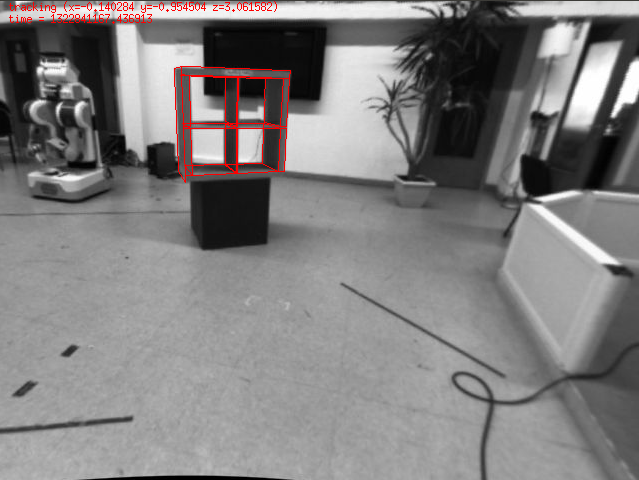
\includegraphics[width=.95\linewidth]{src/chap4-integration/shelf.png}
  \end{center}
  \caption{Le visualisateur associé au composant de suivi d'objet.}
\end{figure}



Il est courant de modéliser le comportement des composants robotiques
sous la forme d'une machine à état. Dans notre cas le composant de
suivi est dans un état ``non initialisé'' au départ où il reçoit déjà
des images et des informations de calibration mais ne réalise aucun
traitement. Un service permet d'initialiser le suivi en fournissant à
la fois la pose initiale de l'objet, son modèle et les paramètres de
suivi. Le n\oe passse alors dans un état actif où il réalise le
suivi. Si le suivi est perdu à un moment ou un autre, le n\oe ud passe
dans un état ``perdu'' où il tente de réinitialiser le suivi avec la
dernière position connue. Si une estimation de la position de la
caméra est disponible, elle va être utilisée pour tenter de fournir
une estimation de la nouvelle position de l'objet en considérant ce
dernier statique. À n'importe quel moment le service d'initialisation
permet de relancer le suivi.


Afin de simplifier l'utilisation du n\oe ud, deux programmes
additionels sont fournis: le premier permet de calculer une pose
initiale de manière graphique. L'utilisateur peut cliquer sur des
points de l'objet prédéfinis et dont on connaît la position relative
en trois dimensions dans l'objet. Cet outil transmet également au
composant de suivi le modèle de l'objet. Le contexte distributé de
l'application empêche de passer directement des emplacements de
fichiers car il n'y a aucune garantie que le composant réalisant le
suivi et le programme réalisant l'initialisation partage leur système
de fichier. Le modèle est donc directement transmis sous sa
représentation textuelle via le réseau. De plus, le composant pouvant
être lancé à distance, laisser l'utilisateur spécifier le chemin vers
le modèle sous la forme d'un chemin local est une mauvaise idée car il
sera tenté d'y insérer le chemin sur sa machine et non sur celle sur
laquelle le composant va être lancé. Pour se faire, l'emplacement du
modèle est passé sous la forme d'une URI -- Uniform Resource
Identifier --~\citep{rfc2396}.


Le second outil permet de surveiller l'état du tracking en affichant
non seulement la reprojection du modèle dans l'image mais surtout
l'état du suivi des lignes du modèle. L'algorithme pouvant rejeter des
points pour différentes raisons, cet outil fournit un retour graphique
de ces informations afin d'aider l'utilisateur à trouver le meilleur
ensemble de paramètres pour optimiser le suivi.


Le dernier point à considérer a été d'intégrer le modèle de
calibration de ROS à ViSP. En effet, ROS annote chaque image avec les
paramètres intrinsèques de caméra. Ces données sont exprimées sous
forme matricielle et doivent être converties avant d'être mises à jour
dans ViSP ce qui nécessite un traitement simple. L'avantage étant que
de cette manière, on peut complètement contourner le processus de
rectification de ViSP qui nécessiterait une calibration spécifique
pour l'utilisation de ce composant.


Les difficultés rencontrées durant cette intégration sont nombreux: il
a fallu supprimer le code interactif, notamment pour calculer la pose
initiale qui nécessite de cliquer sur une image. Un tel code ne peut
pas fonctionner sur le robot. Il a fallu s'abstraire du système de
fichier local afin de rendre le système facilement distribuable et il
a fallu trouver une façon de pouvoir exprimer les informations de
``debug'' de manière minimale. Une solution aurait été de tracer une
image avec le résultat du suivi, mais les robots étant souvent reliés
en wifi à la console le controlant, transmettre un tel flot
d'information n'est pas justifiable. À la place, un topic
supplémentaire pour les développeur a été ajouté. Le défi est alors
d'assurer la cohérence des données entre d'un côté les images
provenant du composant de vision, de la pose provenant du tracker
ainsi que du topic transportant les informations supplémentaire pour
les développeurs. Ces informations sont filtrées afin que seul les
triplets présentant un temps identique soient affichés. En effet, dans
les précédentes versions, cette synchronisation n'était pas
réalisée. On avait alors l'impression que le suivi était de mauvaise
qualité alors que le problème venait simplement de l'affichage. Les
paramètres de tracking sont également modifiables durant l'exécution
afin de simplifier la recherche du meilleur paramétrage. Cela ouvre
également la possibilité pour un composant de plus haut niveau, de
changer le comportement du logiciel de suivi et réaliser de ce fait,
une forme de suivi ``supervisé''. On notera qu'une fois de plus, la
définition des paramètres joue un rôle très important. Ici l'absence
de sens physique de certains d'entre eux est dommageable: par exemple
la recherche de la nouvelle pose se fait dans un voisinage qui est
défini en pixel. En pratique, cela signifie que si l'on se rapproche
de l'objet, l'absence de reconfiguration de ce paramètre va causer
l'échec du suivi. Un meilleure paramètre aurait été de passer par une
borne sur la vitesse maximum de la caméra qui aurait permis d'avoir un
comportement cohérent quelque soit la distance à l'objet.


Au final, ce composant a reçu un accueil favorable de la communauté
avec plusieurs utilisateurs confirmés dans des laboratoires et
sociétés tiers. Ces utilisateurs n'avaient pas d'expérience avec les
techniques d'asservissement visuel avant de tenter d'intégrer ce
composant et ont réussi à obtenir des résultats satisfaisants dans le
cadre de leur utilisation si des robots différents, notamment le robot
REEM de Pal Robotics\footnote{\url{http://www.pal-robotics.com/}}. De
ce fait l'objectif qui consistait à pouvoir maîtriser la complexité de
la mise en place d'un tel méchanisme a été rempli au travers des choix
réalisés ici. Ce composant a pu être utilisé dans le cadre d'une
architecture robotique distribuée sur deux ordinateurs et
l'introduction d'une interface au niveau de la componentisation
robotique a permis au robot HRP-2 de se localiser soit en utilisant ce
composant, soit en utilisant un composant de SLAM, soit encore le
système de capture de mouvement de manière transparente. Seul le
lancement du graphe diffère dans ces trois cas.


\subsubsection{Cycle de développement d'une architecture}


La section précédente a décrit le développement d'un composant en
particulier, mais concevoir une architecture ne revient pas à
simplement dupliquer cette approche autant de fois qu'il y a de
composants nécessaire. Il faut tout d'abord découper le problème en
composants cohérents, puis assigner ces composants à un ordinateur
parmi ceux qui équipent le robot et enfin paramétrer chacun des
composants de manière optimale. Dans la mesure où une approche
modulaire a pour intérêt principale la réutilisabilité des
composants, on sera donc contraint par l'interface des composants
pré-existants que l'on devra réutiliser, ainsi que par les contraintes
matérielles de la plate-forme: les caméras d'HRP-2 sont connectées à
un PC donné donc le composant d'acquisition des images ne peut
fonctionner que sur ce dernier. Inversement, les commandes sont
envoyées via une carte connectée au second PC, le composant de
contrôle ne pourra tourner que sur celui-ci. De plus, le temps réel
contraint le contrôleur a n'être constitué que d'un seul processus. Le
dernier élément à prendre en compte est la communication intra-n\oe
uds: les communications par ``topics'' ou service induisent un retard
qui doit pouvoir être accepté ou géré convenablement. Un autre élément
à prendre en compte est la bande-passante disponible entre les
ordinateurs qui constituent le robot. Il faut s'efforcer de minimiser
la bande pasante consommée entre les ordinateurs. Pour les composants
effectuant de l'affichage ou de la surveillance distant le problème
est souvent encore plus critique dans la mesure où le robot est la
plupart du temps connecté en wi-fi et dispose donc d'un lien avec une
bande-passante extrêmement limitée vers l'extérieur. Cette contrainte
va donc contrainte les composants de perception, la plupart du temps
gros producteurs et consommateurs de donnée, à se situer sur le même
hôte. Une fois le traitement des images terminé, le résultat final
peut représenter un volume d'information bien plus compact:
trajectoire ou position 3d par exemple.


En considérant la répartition des composants sur les différentes
machines, il faut déterminer la liste des composants nécessaire. En
général, on part d'un côté de la liste des capteurs que l'on souhaite
utiliser, que l'on fait communiquer avec les algorithmes utilisant ces
données en entrée qui eux même communique avec la partie
décisionelle. Cette partie étant généralement algorithmique, le
positionement de ces composants n'est pas soumis à des contraintes
techniques fortes. Enfin, un composant de contrôle est nécessaire pour
envoyer les commandes.


Une fois les n\oe uds choisis et paramétrés, l'étape suivante est la
simulation. De nombreux outils permettent de simuler un mouvement
dynamique dans un monde virtuel. Il est nécessaire ici de remplacer
les composants réalisant l'acquisition des données capteurs par des
composants acccédant aux informations équilvalentes simulées et le
contrôleur par un contrôleur envoyant sa commande au simulateur. Une
phase supplémentaire de définition du monde est souvent nécessaire.


Une fois validée en simulation, l'architecture est portée sur le robot
proprement dit. On peut alors faire tourner l'architecture sans
envoyer réellement les commandes aux actionneurs afin de vérifier
l'accès aux données capteurs, les délais induits par les
communications entre les hôtes, etc. Enfin, l'architecture peut être
testée réellement en validant plusieurs scénarii adaptés de difficulté
croissante. Une fois l'expérience validée, on peut alors changer
certains composants afin de tester de nouvelles stratégies ce qui fait
débuter un nouveau cycle comme illustré sur la figure FIXME.


\begin{figure}
  \begin{center}
    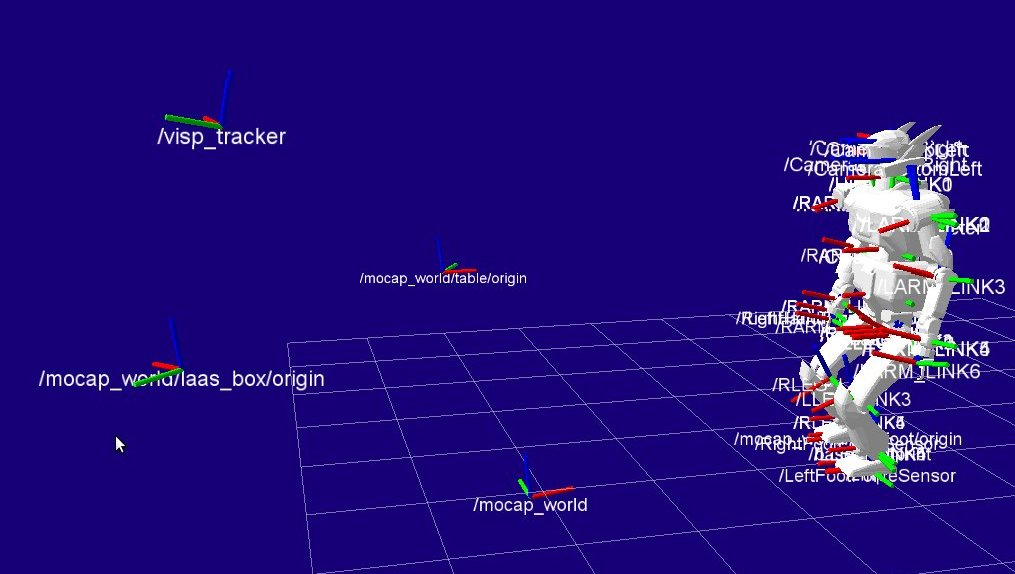
\includegraphics[width=.95\linewidth]{src/chap4-integration/rviz-full.jpg}
  \end{center}
  \caption{Architecture complexe associant de nombreux composants
    robotiques intégrant le contrôleur du robot exécutant une tâche de
    locomotion, le système de capture de mouvement et le processus
    complet de vision utilisant le tracker décrit dans cette section
    pour estimer la position d'un cube.}
\end{figure}



\section{Conclusion}


Construire une architecture robotique est une tâche ardue, non
seulement parce qu'elle aggrège des algorithmes complexes, mais
surtout parce qu'il est nécessaire de considérer la plate-forme
utilisée et les problèmes techniques qui lui sont propres -- délais,
puissance de calcul disponible --, afin de construire un ensemble
fonctionnel. Cette section a donc à la fois présenté comment
développer un composant robotique puis comment combiner plusieurs
composants pour réaliser une architecture. Les différentes difficultés
inhérentes à la conception d'un système complexe ont été passées en
revue ainsi que les stratégies qui ont été adoptées au cours de ces
trois années. Il est probable qu'au cours des prochaines années de
nombreuses architectures robotiques complexes voient le jour sur des
robots humanoïdes afin de le rendre sensible à l'évolution de
l'environnement qui les entoure. Un objectif ambitieux pour lequel les
robots mobiles restent la plate-forme d'expérimentation principale
dans l'état actuel de la littérature.


